\chapter{unendliche Dimension}
\label{sec:unendliche VRs}

\section{Funktionenvektorraum}
\theoremstyle{Satz}
\begin{Satz}{Der reelle Funktionenraum}
\label{funktionenraum}
\\ Die Menge aller reellen Funktion \[F :=  \Abb(\mathbb{R}, \mathbb{R}):= \{f : \mathbb{R} \rightarrow\mathbb{R}\}\]
bilden einen \acl{VR} über den Körper der reellen Zahlen $\mathbb{R}$ mit folgender Definition von Addition und Skalarmultiplikation:
\begin{enumerate}
	\item Die Addition $f+g\in F$ für $f,g \in F$ definieren wie als 
	
	\begin{align} (f+g)(x) := f(x)+ g(x)\text{.} \label{funkadd}
	\end{align}
	
	\item Die Skalarmultiplikation $\lambda \cdot f \in F$ für $\lambda \in \mathbb{R}$ und $f \in F$ definieren wir als 
	
	\begin{align}(\lambda \cdot f)(x) := \lambda \cdot f (x)\text{.}\label{funkskalmult} 
	\end{align}
		
\end{enumerate}
\end{Satz}

\begin{proof}
Vor.: Funktionenaddition von \ref{funkadd} und Funktionenskalarmultiplikation von \ref{funkskalmult} werden für alle Beweise benötigt.
\\ Beh.: $F$ ist ein $\mathbb{R}$-\acl{VR}.
\\ Bew.: Wir müssen $F$ auf alle Vektorraumaxiome (siehe \ref{VR-axiome}) hin überprüfen. Aus der Definition von $F$ folgt: \(f(x) \in \mathbb{R}\) für alle $f$. Die Ergebnisse aller Funktionen aus $F$ sind reelle Zahlen, somit haben sie alle Körpereigenschaften (siehe \ref{Koerper}). Wir können mit ihnen wie gewohnt rechnen.
\\Zuerst zeigen wir, dass $(F,+)$ eine abelsche Gruppe (vgl. \ref{Gruppe}, \ref{abl.Gruppe}) ist.
\\
\\
\\Für alle $f,g,h \in F$ und $\lambda_1, \lambda_2 \in \mathbb{R}$ gilt:
\begin{enumerate}
\item (Assoziativität)
\(((f+g)+h)(x)=(f+g)(x)+h(x)=f(x)+g(x)+h(x)=\\f(x)+(g(x)+h(x))=(f+(g+h))(x)\)
\item(Existenz des neutralen Elements) Sei $0_{\Abb}(x)=0$ für alle $x \in \mathbb{R}$.\footnote{Wir bezeichnen diese Funktion als die sogenannte "Nullabbildung", die alle Elemente auf $0$ abbildet. Ihr Graph ist die $x$-Achse.} \\ \( (0_{\Abb}+f)(x) = 0_{\Abb}(x) + f(x)= 0+ f(x)=f(x)=f(x)+0=f(x)+ 0_{\Abb}(x)=(f+0_{\Abb})(x) \)
\item(Existenz des Inversen) Sei $-f \in F$ das Inverse für alle $f\in F$.\\ \( (f+(-f))(x) =  f(x) + (-f(x))= f(x)-f(x) = 0_{\Abb}(x) =  (-f(x)) + f(x)= ((-f) + f)(x)\) 
\item(Kommutativität) \((f+g)(x)=f(x)+g(x)=g(x)+f(x)=(g+f)(x)\)
\end{enumerate}

Es müssen noch die Eigenschaften eines \acl{VR}es gezeigt werden.
\begin{enumerate}
\item \((\lambda_1+\lambda_2)\cdot f(x) = \lambda_1 \cdot f(x) + \lambda_2 \cdot  f(x)\)
\item \( \lambda_1 \cdot (f + g)(x) = (\lambda_1 \cdot f + \lambda_1 \cdot  g)(x) = \lambda_1 \cdot f(x) + \lambda_1 \cdot  g(x)\)
\item \( \lambda_1 \cdot (\lambda_2 \cdot f(x)) = (\lambda_1 \cdot \lambda_2) \cdot f(x) \)
\item \(1 \cdot f(x) = f(x)\)
\end{enumerate}
\end{proof}
\newpage


%\theoremstyle{example}
%\begin{example}{Funktionenaddition}
\begin{figure}[h]
\begin{minipage}[h]{.5\textwidth}
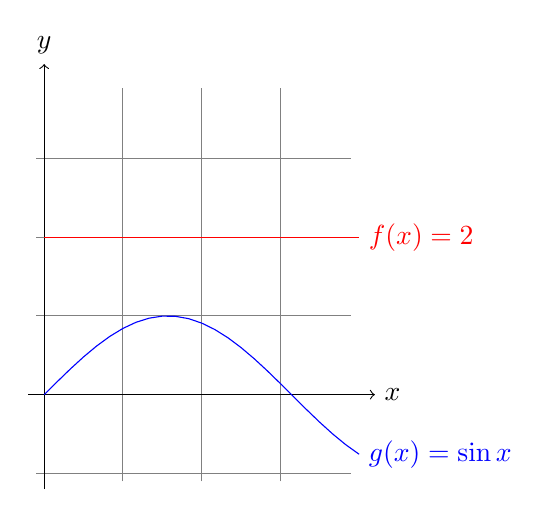
\begin{tikzpicture}[domain=0:4] 
	\draw[color=gray] (-0.1,-1.1) grid (3.9,3.9);
	\draw[->] (-0.2,0) -- (4.2,0) node[right] {$x$}; 
	\draw[->] (0,-1.2) -- (0,4.2) node[above] {$y$};
	\draw[color=red] plot (\x,2) node[right] {$f(x) =2$}; % \x r means to convert ’\x’ from degrees to _r_adians: 
	\draw[color=blue] plot (\x,{sin(\x r)}) node[right] {$g(x) = \sin x$}; 
\end{tikzpicture}
\captionsetup{singlelinecheck=off}
\caption{}
\end{minipage}
\hfil
\begin{minipage}[h]{.5\textwidth}
\begin{tikzpicture}[domain=0:4] 
	\draw[color=gray] (-0.1,-1.1) grid (3.9,3.9);
	\draw[->] (-0.2,0) -- (4.2,0) node[right] {$x$}; 
	\draw[->] (0,-1.2) -- (0,4.2) node[above] {$y$};
	 % \x r means to convert ’\x’ from degrees to _r_adians: 
	\draw[color=violet] plot (\x,{sin(\x r)+2}) node[right] {$(f+g)(x) = 2+\sin x$}; 
\end{tikzpicture}
\captionsetup{singlelinecheck=off}
\caption{}
\end{minipage}
\end{figure}

\begin{tikzpicture}[domain=0:4] 
	\draw[color=gray] (-0.1,-1.1) grid (3.9,3.9);
	\draw[->] (-0.2,0) -- (4.2,0) node[right] {$x$}; 
	\draw[->] (0,-1.2) -- (0,4.2) node[above] {$y$};
	\draw[color=blue] plot (\x,{2*sin(\x r)}) node[right] {$2 \cdot f(x) =2 \cdot \sin x$}; 
\end{tikzpicture}

\section{Polynomvektorraum}
\label{sec:RX}
Wir wollen uns mit einer spezifischeren "Gattung" von reellen Funktionen beschäftigen, nämlich den \emph{Polynomen}.

\theoremstyle{definition}
\begin{definition}{\textbf{Polynome}}
\label{def:Polynome}
\\Ein Polynom vom Grad $\leq n$ hat die Form \[f(x)= \sum\limits_{i=0}^{n} \lambda_i x^i = \lambda_0 + \lambda_2 x^1 + ... + \lambda_n x^n \] für $\lambda_i \in \mathbb{R}$ (vgl. \cite[S. 44, 1.28]{Springer}) .\footnote{Zur Erinnerung: Beachte, dass $x^0 = 1$ und $x^1=x$ ist.}
\end{definition}

\theoremstyle{Satz}
\begin{Satz}{\emph{Polynomvektorraum} $\mathbb{R}[x]$}
\label{PV}
\\ Die Menge aller Polynome aus \ref{def:Polynome} bezeichnen wir als $\mathbb{R}[x]$. Sie bildet einen $\mathbb{R}$-\acl{VR} mit der Definition von Addition und Multiplikation aus \ref{funktionenraum}:
\begin{enumerate}

\item (Polynomaddition) Für alle \(f(x)=\sum\limits_{i=0}^{n} \mu_i x^i\text{,}\; g(x)=\sum \limits_{i=0}^n \nu_i x^i\) gilt:
\begin{align}(f+g)(x) = \sum_{i=0}^{n}\mu_i x^i + \sum_{i=0}^{n} \nu_i x^i = \sum_{i=0}^{n} (\mu_i + \nu_i)x^i \text{.}\end{align}
\item (Polynomskalarmultiplikation)
Seien $f(x) \in \acl{RX}$ beliebig und $c \in \mathbb{R}$.
\begin{align}
(c \cdot f) (x) = c \cdot \sum_{i=0}^{n} \mu_i x^i= \sum_{i=0}^{n} c \cdot \mu_i x^i\text{.}
\end{align}
\end{enumerate}
(vgl. \cite[S. 44f., 1.28]{Springer})
\end{Satz}

\theoremstyle{Corollar}
\begin{Corollar}
\label{PV ist UVR}
Der Polynomvektorraum ist ein \acl{UVR} (siehe \ref{UVR}) von $F$.
\end{Corollar}

\begin{proof}
Vor.: Plynomaddition und -skalarmultiplikation aus \ref{PV}.
\\ Beh.: siehe \ref{PV ist UVR}
\\ Bew.: Wir rechnen die Axiome aus \ref{UVR} für $\acl{RX}$ durch.
\\ Seien $u(x)=\sum\limits_{i=0}^{n} \zeta_i x^i\text{,}\; v(x) = \sum\limits_{i=0}^{n} \eta_i x^i \in \acl{RX}$ beliebig.
\begin{enumerate}
\item Zu zeigen gilt, dass der Nullvektor ein Element von $\acl{RX}$ ist. Sei $\rho = 0$. \[\rho \cdot u(x)= 0 \cdot \sum\limits_{i=0}^{n} \zeta_i x^i = 0 \Rightarrow 0 \in \acl{RX}\]
\item Es gilt die Ageschlossenheit\footnote{Abgelossenheit bezeichnet die Eigenschaft nach einer Verknüpfung beliebiger Elemente einer Menge wie Skalarmultiplikation und Vektoraddition wieder ein Element derselben Menge zu sein.} der Polynomaddition zu beweisen.
\\ \[ (u+v)(x)=u(x) + v(x) = \sum\limits_{i=0}^{n} \zeta_i x^i+\sum\limits_{i=0}^{n} \eta_i x^i =\sum\limits_{i=0}^{n} (\zeta_i+ \eta_i )x^i \in \acl{RX} \]
\item Die Skalarmultiplikation soll auf ihre Abgeschlossenheit getestet werden. Sei $\varrho \in \acl{RX}$ frei wählbar.
\[(\varrho \cdot u)(x) = \varrho \cdot u(x)= \varrho \cdot \sum\limits_{i=0}^{n} \zeta_i x^i\ = \sum\limits_{i=0}^{n} \varrho \cdot \zeta_i x^i \in \acl{RX}\]
\end{enumerate}
\end{proof}

\subsection*{Basis $\acl{RX}$}

%Wir benötigen eine Basis, um die Dimension des \acl{PV}es zu bestimmen. 
\theoremstyle{Lemma}
\begin{Lemma}{\emph{Basis von $\acl{RX}$}}
\\ Die Menge der Monome $\{1, x, x^2,…, x^n\}$ vom Grad $\leq n$ bildet eine Basis $B_{\acl{RX}}$ des \acl{PV}. 
\end{Lemma}

\begin{proof}
\label{BewBas}
Vor.: Theo. \ref{theo:Basis} (\ref{Basis1}), Def. \ref{def:Polynome}, Def. \ref{def:linunab}
\\ Beh.: $B_{\acl{RX}}:=\{1, x, x^2,…, x^n\}$ sei eine Basis des Polynomvektorraums.
\\ Bew.: Wir müssen überprüfen, ob die Menge \acl{linunab} und ein \acl{EZS} ist.  
\\ \acl{Linunab}:
\\ Es ist zu zeigen, dass die Gleichung \begin{equation}\label{GLS} \sum\limits_{i=0}^n \lambda_i x^i = \lambda_i x^i = \lambda_0 + \lambda_1 x^1 + ... + \lambda_n x^n = 0\end{equation} nur für alle $\lambda_i=0$ mit $i \in \mathbb{N}_0$ lösbar ist.\footnote{Wir müssen ein Gleichungssystestem mit $n$ Variablen schrittweise lösen. Dies erfolgt durch "geschickt gewählte $x$" (vgl. \cite[S. 308]{Tut}).}
\begin{enumerate}
\item \label{S1} Setze zunächst $x=0$ in (\ref{GLS}). 
\begin{equation}\Rightarrow \lambda_0 + \lambda_1 \cdot 0 + \lambda_2 \cdot 0^2 + ... + \lambda_n \cdot 0^n\ \Rightarrow \lambda_0 = 0 \end{equation}
\item Setze $\lambda_0$ in (\ref{GLS}) ein. 
\begin{align}
\label{GLS2} 
\lambda_1 \cdot x + \lambda_2 \cdot x^2+ ... + \lambda_n \cdot x^{n-1} = 0 
\end{align} Wir dürfen (\ref{GLS2}) nun durch $x$ teilen, wenn $x\not= 0$ ist: 
\begin{align}
\lambda_1 \cdot x + \lambda_2 \cdot x^2 +... + \lambda_n  \cdot x^n &= 0 && |:x \\ \Rightarrow \lambda_1 + \lambda_2 \cdot x^2+ ... + \lambda_n \cdot x^{n-1} &= 0
\end{align}
\end{enumerate}
Wiederhole (\ref{S1}), (\ref{GLS2}), bis wir nacheinander erhalten, dass alle $\lambda_i=0$ mit $i \in \mathbb{N}_0$ sind.
Somit ist die \acl{Linunab} von $B_{\acl{RX}}$ gezeigt. (vgl. \cite[S. 308]{Tut}) \qed
\\
\\ \acl{EZS}: Aus Def. \ref{def:Polynome} ist ersichtlich, dass jede Polynomfunktion $f(x)$ eine Linearkombination der Monome $1, x,x^2 …, x^n$ vom Grad $\leq n$ ist. Folglich bildet $B_{\acl{RX}}$ ein \acl{EZS}.
\end{proof}

\section{unendlichdimensionale \aclp{VR}}
\subsection*{unendliches \acl{EZS}}

\theoremstyle{prop}
\begin{prop} \label{propunendl}$\acl{RX}$ hat ein "unendliches \acl{EZS}" \cite[S.498 f.]{Enzy} $B_{\acl{RX}}=\{1,x,x^2,...,x^n\}$ mit $n \in \mathbb{N}_0$.
\end{prop}


\begin{proof}
Nun wollen wir mit einem Widerspruchsbeweis zeigen, dass das System $B_{\acl{RX}}$ unendlich erzeugt ist.
\\Vor.: Im vorigen Beweis wurde bereits überprüft, dass $B_{\acl{RX}}$ ein \textbf{\acl{EZS}} ist. 
\\Beh.: Siehe Prop. \ref{propunendl}.
\\Bew.: Angenommen, $B_{\acl{RX}}$ sei ein endliches \acl{EZS}. Somit gibt es ein Polynom vom maximalen Grad $n$. Das "nächsthöhergradige" Polynom vom Grad $n+1$ lässt sich allerdings nicht mehr durch eine \acl{Linkomb} von $B_{\acl{RX}}$ darstellen. Dies ist ein Widerspruch dazu, dass $B_{\acl{RX}}$ ein \textbf{\acl{EZS}} ist (vgl.  \cite[S.498 f.]{Enzy}).\footnote{$\acl{BRX}$ müsste alle Polynome "linear kombinieren" können.} So folgt die Behauptung.
\end{proof}

\theoremstyle{Corollar}
\begin{Corollar}{ }
Aus der Definition des Dimensionenbegriffs in \ref{def:dim} schließen wir aufgrund des unendlichen \acl{EZS}s von $\acl{BRX}$, dass $\dim(F)= \infty$ ist. 
\end{Corollar}

\subsection*{abzählbar unendliche Dimension}
Wir wollen die Kardinalität der Unendlichkeit in diesem Falle untersuchen.

\theoremstyle{prop}
\begin{prop}{ }
Die Dimension des reellen Polynomvektorraumes $\acl{RX}$ lautet: \begin{align*}\dim(\acl{RX})=\aleph_0\text{.} \end{align*}
\end{prop}

\begin{proof}
Vor.: Aus dem W-Seminarunterricht wissen wir, dass eine Menge $M$ genau dann abzählbar ist, wenn $|M|=|\mathbb{N}_0|=\aleph_0$ gilt.
\\Beh.: $\acl{BRX}$ ist abzählbar.
\\Bew.: Wir konstruieren eine eineindeutige\footnote{Zur Erinnerung: Jedem Element wir genau ein Element aus der Wertemenge zugeordnet. Wir sagen stattdessen uauch "bijektiv".} Funktion: Sei $n \in \mathbb{N}_0$.
\begin{align}
\alpha: \acl{BRX} &\rightarrow \mathbb{N}_0
\\ x^n &\mapsto n \end{align}
$\Rightarrow |\acl{BRX}|=\aleph_0 \Rightarrow \dim(\acl{RX})=\aleph_0$ 
\end{proof}

\subsection*{überabzählbar unendliche Dimension}
Wir wollen im Folgenden berechnen, welche Dimension $F$ hat. Da wir wissen, dass $\acl{RX}$ ein \acl{UVR} von $F$ ist, muss $\dim(F)\geq\acl{RX}$ sein.









